\documentclass[tikz,border=8pt]{standalone}
% Shared look for every TikZ diagram. Load with \input{../../tools/tikz-style.tex}
\usepackage[sfdefault]{roboto}
\usetikzlibrary{arrows.meta, positioning, shapes.geometric, calc, fit, backgrounds}
\definecolor{cblue}{HTML}{4C78A8}
\definecolor{corange}{HTML}{F58518}
\definecolor{cgreen}{HTML}{54A24B}
\definecolor{cred}{HTML}{E45756}
\definecolor{cpurple}{HTML}{B279A2}
\definecolor{cgrey}{HTML}{6B6B6B}
\tikzset{
  every picture/.style={font=\sffamily, line width=1.2pt},
  box/.style={draw=#1, fill=#1!12, rounded corners=4pt, align=center, inner sep=7pt, minimum height=1.1cm},
  box/.default=cgrey,
  arrow/.style={-{Stealth[length=3mm]}, draw=cgrey, line width=1.4pt},
  title/.style={font=\sffamily\bfseries\Large},
  note/.style={font=\sffamily\small, text=cgrey, align=center},
}
\AtBeginDocument{\hyphenpenalty=10000 \exhyphenpenalty=10000}

% Left: the 8 moves from a cell of the 0.5 m grid: 4 straight moves of 0.5 m and 4 diagonal moves of 0.707 m.
% Middle: the diagonal is the long side of a right-angled triangle with two 0.5 m sides. Right: a diagonal move
% that would cut the corner of a blocked cell is not allowed, because the robot would clip the blocked cell.
\begin{document}
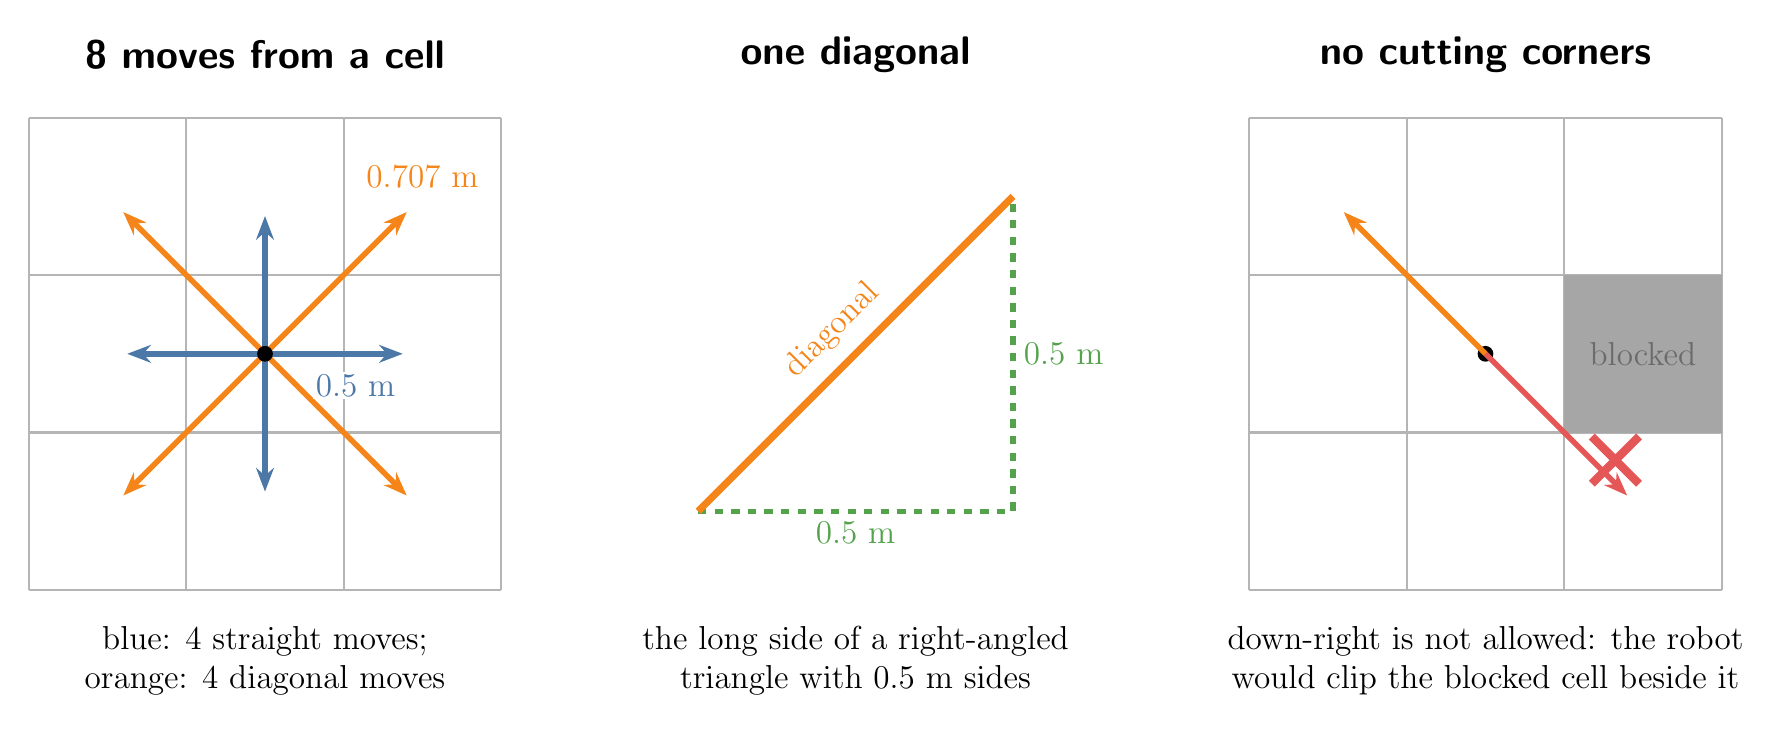
\begin{tikzpicture}[every node/.append style={font=\large}]
  % left panel: 3 x 3 cells of 0.5 m, drawn 2 units wide
  \node[title] at (3,6.8) {8 moves from a cell};
  \draw[cgrey!50, line width=0.8pt] (0,0) grid[step=2] (6,6);
  \foreach \dx/\dy in {1/0,-1/0,0/1,0/-1} \draw[-{Stealth[length=3mm]}, cblue, line width=2pt] (3,3) -- ++(1.75*\dx,1.75*\dy);
  \foreach \dx/\dy in {1/1,-1/1,1/-1,-1/-1} \draw[-{Stealth[length=3mm]}, corange, line width=2pt] (3,3) -- ++(1.8*\dx,1.8*\dy);
  \fill[black] (3,3) circle (0.1);
  \node[cblue, fill=white, inner sep=1pt] at (4.15,2.6) {0.5 m};
  \node[corange, fill=white, inner sep=1pt] at (5.0,5.25) {0.707 m};
  \node[align=center] at (3,-0.9) {blue: 4 straight moves;\\orange: 4 diagonal moves};
  % middle panel: the triangle
  \begin{scope}[xshift=8.5cm]
    \node[title] at (2,6.8) {one diagonal};
    \draw[cgreen, line width=2pt, dashed] (0,1) -- (4,1) -- (4,5);
    \draw[corange, line width=2.5pt] (0,1) -- (4,5);
    \node[cgreen, below] at (2,1) {0.5 m};
    \node[cgreen, right] at (4,3) {0.5 m};
    \node[corange, fill=white, inner sep=1pt, rotate=45] at (1.7,3.3) {diagonal};
    \node[align=center] at (2,-0.9) {the long side of a right-angled\\triangle with 0.5 m sides};
  \end{scope}
  % right panel: corner cutting
  \begin{scope}[xshift=15.5cm]
    \node[title] at (3,6.8) {no cutting corners};
    \draw[cgrey!50, line width=0.8pt] (0,0) grid[step=2] (6,6);
    \fill[cgrey!60] (4,2) rectangle (6,4);
    \node[cgrey] at (5,3) {blocked};
    \fill[black] (3,3) circle (0.1);
    \draw[-{Stealth[length=3mm]}, cred, line width=2pt] (3,3) -- (4.8,1.2);
    \draw[cred, line width=3pt] (4.35,1.35) -- (4.95,1.95) (4.35,1.95) -- (4.95,1.35);
    \draw[-{Stealth[length=3mm]}, corange, line width=2pt] (3,3) -- (1.2,4.8);
    \node[align=center] at (3,-0.9) {down-right is not allowed: the robot\\would clip the blocked cell beside it};
  \end{scope}
\end{tikzpicture}
\end{document}
